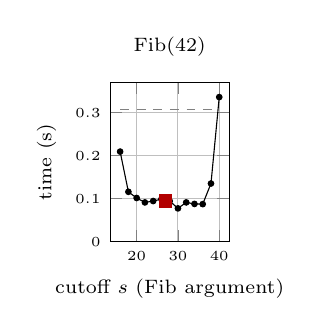
\begin{tikzpicture}
\begin{axis}[width=0.255\textwidth,height=3.6cm,title={\scriptsize Fib(42)},xlabel={\scriptsize cutoff $s$ (Fib argument)},
 ylabel={\scriptsize time (s)},tick label style={font=\tiny},grid=major,ymin=0]
\addplot[black,mark=*,mark size=1pt] coordinates {(16,0.2095) (18,0.1159) (20,0.1015) (22,0.0912) (24,0.0944) (26,0.0989) (28,0.0944) (30,0.0773) (32,0.0912) (34,0.0877) (36,0.0872) (38,0.1352) (40,0.3364)};
\addplot[only marks,mark=square*,mark size=2.2pt,red!70!black] coordinates {(27,0.0946)};
\addplot[gray,dashed,domain=16:40] {0.3068};
\end{axis}
\end{tikzpicture}\hfill
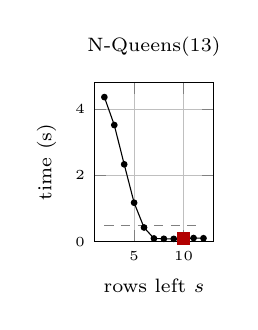
\begin{tikzpicture}
\begin{axis}[width=0.255\textwidth,height=3.6cm,title={\scriptsize N-Queens(13)},xlabel={\scriptsize rows left $s$},
 ylabel={\scriptsize time (s)},tick label style={font=\tiny},grid=major,ymin=0]
\addplot[black,mark=*,mark size=1pt] coordinates {(2,4.3610) (3,3.5178) (4,2.3321) (5,1.1730) (6,0.4254) (7,0.0950) (8,0.0840) (9,0.0820) (10,0.0800) (11,0.1074) (12,0.1009)};
\addplot[only marks,mark=square*,mark size=2.2pt,red!70!black] coordinates {(10,0.0892)};
\addplot[gray,dashed,domain=2:12] {0.4887};
\end{axis}
\end{tikzpicture}\hfill
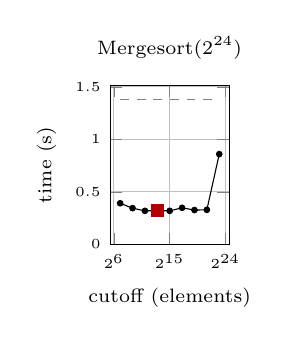
\begin{tikzpicture}
\begin{semilogxaxis}[width=0.255\textwidth,height=3.6cm,title={\scriptsize Mergesort($2^{24}$)},xlabel={\scriptsize cutoff (elements)},
 ylabel={\scriptsize time (s)},tick label style={font=\tiny},grid=major,ymin=0,log basis x=2]
\addplot[black,mark=*,mark size=1pt] coordinates {(128,0.3911) (512,0.3445) (2048,0.3188) (8192,0.3206) (32768,0.3191) (131072,0.3476) (524288,0.3265) (2097152,0.3286) (8388608,0.8592)};
\addplot[only marks,mark=square*,mark size=2.2pt,red!70!black] coordinates {(8192,0.3205)};
\addplot[gray,dashed,domain=128:8388608] {1.3760};
\end{semilogxaxis}
\end{tikzpicture}\hfill
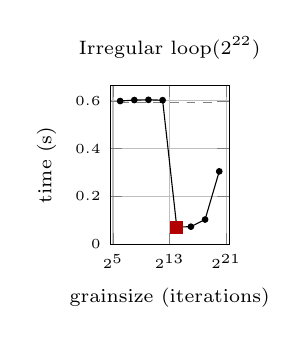
\begin{tikzpicture}
\begin{semilogxaxis}[width=0.255\textwidth,height=3.6cm,title={\scriptsize Irregular loop($2^{22}$)},xlabel={\scriptsize grainsize (iterations)},
 ylabel={\scriptsize time (s)},tick label style={font=\tiny},grid=major,ymin=0,log basis x=2]
\addplot[black,mark=*,mark size=1pt] coordinates {(64,0.5993) (256,0.6033) (1024,0.6042) (4096,0.6028) (16384,0.0723) (65536,0.0738) (262144,0.1037) (1048576,0.3051)};
\addplot[only marks,mark=square*,mark size=2.2pt,red!70!black] coordinates {(15447,0.0707)};
\addplot[gray,dashed,domain=64:1048576] {0.5937};
\end{semilogxaxis}
\end{tikzpicture}
